\documentclass{article}

% Packages
\usepackage{packages}
\usepackage{commands}
\usepackage{titlepage}


% Title page parameters
\setUDK{612.8:[004.93+515.1]}
\setToResearch
\setTitle{Анализ аффективных компонентов ЭЭГ при прослушивании музыки}
\setStageOne
\setGroup{207}
\setStudentSgn{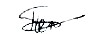
\includegraphics{my_sgn}}
\setStudent{А.С.Петелин}
\setStudentDate{08.02.2022}
\setAdvisor{Всеволод Леонидович Чернышев}
\setAdvisorTitle{доцент, к.ф.-м.н.}
\setAdvisorAffiliation{ФКН НИУ ВШЭ, Департамент больших данных и информационного поиска}
\setAdvisorDate{18.02}
\setGrade{}
\setAdvisorSgn{}
\setYear{2022}


% Document Beginning
\begin{document}

\makeTitlePage
{
  \hypersetup{linkcolor=black}
  \tableofcontents
}

\section{Основные термины и определения}

% Возможно здесь необходимо будет привести ссылки на источники определений?

\textbf{Электроэнцефалограмма} (далее \textbf{ЭЭГ/EEG}) -- один из методов, позволяющих провести исследование головного мозга человека; в основе метода лежит регистрация электрических импульсов от мозга или каких-то его отдельных областей с помощью специального прибора.

\textbf{Центральная нервная система} (далее \textbf{ЦНС}) -- совокупность связанных между собой нейронов, у человека представлена головным и спинным мозгом.

\textbf{Отбор признаков / Feature Selection} (далее \textbf{FS}) -- это оценка значимости признаков модели с помощью алгоритмов машинного обучения с целью сокращения размерности исследуемого пространства.

\textbf{Метод главных компонент / Principle Component Analysis} (далее \textbf{PCA}) -- один из основных методов уменьшения размерности данных при минимизации потерь содержащейся в данных информации.

\textbf{Метод k-ближайших соседей / k-nearest neighbors} (далее \textbf{k-NN}) -- метрический алгоритм для автоматической классификации объектов или регрессии, основанный на оценивании сходства объектов.

\textbf{Топологический анализ данных / Toplological Data Analysis} (далее \textbf{TDA}) -- подход к анализу данных с использованием методов топологии, связанный, прежде всего с извлечением информации из многомерных, неполных и зашумленных наборов данных.

\textbf{Датасет / Data Set} -- (размеченный) набор данных в табличном виде.

\textbf{DEAPdataset} -- датасет для анализа эмоций с данными ЭЭГ, физиологических и видеосигналов.


\section{Введение}
Влияние музыки на слушателей отражено во многих источниках, как в художественных, так и в научных. Так, исследования показывают, что музыка помогает облегчить боль~\cite{Newbold}, влияет на координацию движений~\cite{Repp}~\cite{Aschersleben} и темпы дыхания~\cite{Siwiak}. Также одним из важнейших свойств музыки является её способность влиять на эмоциональное состояние человека~\cite{Koelsch}. Вопрос влияния на эмоциональное состояние человека является одним из ключевых при разработке систем взаимодействия человека и компьютера, более того, подбор подходящей музыки может улучшить состояние отдельного человека при использовании музыкального приложения~\cite{Leslie}. Примером компании, основавшей на этом позитивном изменении свою бизнес модель, является Endel~\cite{Endel}, разработавшая одноимённое приложение. Приложение предлагает персонализированные аудиотреки, которые ``помогут сосредоточиться, расслабиться и уснуть''.

Возрастающий интерес к музыкальной сфере как со стороны бизнеса, так и со стороны отдельных пользователей, позволяет говорить об актуальности изучения взаимодействия человека и музыки. Таким образом, можно поставить задачу распознавания влияния музыки на эмоциональное состояние человека. 

Для изучения влияния музыки прежде всего необходимо его измерить. В настоящий момент существует несколько технологий для фиксирования изменений эмоций, среди которых распознование эмоций по мимике (facial recognition), изучение переферийных физиологических сигналов, а также сигналов мозга. В данном иссследовании мы сосредоточимся на изучении данных о сигналах мозга, полученных с помощью ЭЭГ. Стоит отметить, что характеристики ЭЭГ содержат множество нелинейных зависимостей~\cite{Wang}, что позволяет в дальнейшем поставить вопрос об эффективности различных алгоритмов анализа данных. 

При переходе от этапа сбора данных к оцениванию, исследователи сталкиваются с рядом вопросов: как разбить данные? как сократить их размерность? каким образом классифицировать данные? Для решения этих проблем в машинном обучении существует множество подходов, однако некоторые подходы, не связанные напрямую с машинным обучением, открывают новые возможности решении задач FS и классификации. Одним из таких подходов является TDA -- совокупность методов, основанных на применении топологического анализа. 

Эффективность применения топологических методов в решении обозначенных выше проблем мало изучена, поэтому актуальным вопросом является сравнение рапространённых и проверенных алгоритмов машинного обучения с непривычным для исследователей в этой области топологическим подходом. В соответствии с поставленной задачей можно выделить следующие цели исследования:
\begin{enumerate}
\item Подготовить данные на основе одного из открытых датасетов;
\item Выбрать алгоритм FS для сокращения размерности пространства данных и выделения ключевых признаков будущей модели;
\item Построить классификатор на основе алгоритмов машинного обучения;
\item Изучить топологическую структуру данных и построить топологический классификатор;
\item Сравнить эффективность обоих подходов, выявить взаимосвязи между характеристиками данных и эффективностью рассмотренных алгоритмов.
\end{enumerate}

Ожидаемыми результатами работы станут сведения о применимости обоих рассмотренных подходов и их сравнительная характеристика. Изучив эффективность различных алгоритмов, можно будет в дальнейшем получить преимущество как при иссследованиях, так и при разработке музыкальных сервисов.

\section{Обзор используемых источников и методов}
Предпологается, что работа будет основана на исследовании открытого датасета DEAP, содержащего данные ЭЭГ и некоторые другие сведения, позволяющие изучать эмоции человека во время прослушивания музыки~\cite{Koelstra}. Сравнение некоторых алгоритмов машинного обучения для распознавания эмоций уже приведено в статье~\cite{Nawaz}, более того, авторы статей~\cite{Tandle}, \cite{Scherer} рассказывают ещё больше об исследовании данных ЭЭГ. С другой стороны, в статьях~\cite{Umeda}, \cite{Otter} выдвигается тезис об эффективности алгоритмов TDA для анализа данных. Авторы~\cite{Otter} ссылаются на данные об эффективности применения TDA в некоторых смежных областях, таких как исследования периодичности во временных рядах~\cite{Perea}, анализ естественного языка~\cite{Zhu}, также отмечено, что TDA имеет приложения в нейронауках (\cite{Curto}, \cite{Lord}). В данном исследовании предлагается изучить возможность применения алгоритмов, основанных на TDA для исследования влияния музыки на эмоциональное состояние человека.

% Bibliography
\bibliographystyle{plainurl}
\bibliography{bibl}

\section*{Приложение А. Календарный план работ}
\addcontentsline{toc}{section}{Приложение А. Календарный план работ}

\setlength{\tabcolsep}{18pt}
\renewcommand{\arraystretch}{1.5}
\begin{tabular}{|m{10cm}|m{5cm}|}
    \hline
    \textbf{Этап работы} & \textbf{Предполагаемые даты}\\
    \hline
    КТ1. Загрузка исправленного с учетом замечаний Отчета с подписанным студентом титульным листом & Не позднее 17.02.22\\
    \hline
    КТ1. Оценивание результатов и передача оценки в ЦППРиП & Не позднее 22.02.22\\
    \hline
    Представление результатов выполнения Проекта руководителю & Не позднее, чем за 10 рабочих дней до даты защиты\\
    \hline
    Подготовка и представление руководителю итогового варианта результатов Проекта & Не позднее, чем за 6 рабочих дней до даты защиты\\
    \hline
    Загрузка итогового варианта Проекта в SmartLMS/LMS для проверки работы в системе «Антиплагиат» & Не позднее, чем за 6 рабочих дней до даты защиты\\
    \hline
    Отзыв руководителя & Не позднее, чем за 3 рабочих дня до даты защиты\\
    \hline
    Загрузка в Задание дисциплины «Программный проект для студентов 2 курса ПМИ» в SmartLMS итогового варианта Проекта, отзыва руководителя, отчета системы “Антиплагиат”, других необходимых материалов & Не позднее, чем за 3 рабочих дня до даты защиты\\
    \hline
    Публичная защита Проекта & Согласно утвержденному графику\\
    \hline  
\end{tabular}

\end{document}
